\chapter{Tecnologie}
In questo capitolo verranno descritte le attività preliminari per la realizzazione di questo progetto, le tecnologie utilizzate
unitamente alle motivazioni legate all'uso di questi sistemi rispetto ad altri.

\section{Strutture dati gerarchiche}
Le tabelle di un database relazione non sono gerarchiche (come nel XML), ma sono delle semplici liste piatte. I dati gerarchici sono 
constituiti da relazioni padre-figlio che non possono essere rappresentate in modo naturale nelle tabelle dei database relazionali.
In questo caso, i dati gerarchici sono una collezione di informazioni dove ogni item ha un solo padre e nessuno o più figli
(ad eccezione del nodo radice che non ha un nodo padre); questo genere di rappresentazione delle informazioni può essere trovato in 
diversi ambiti di applicazione di un database, incluse discussioni su forum e mailing list, grafici di organizzazione di un business, 
categorie per gestire contenuti e categorie di prodotti. 

\begin{figure}[H]
	\label{fig:Hde}
	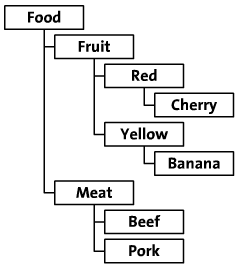
\includegraphics[scale=0.45]{images/Hierarchical_Data_ex.PNG}
	\caption{Esempio di una gestione di dati in modo gerarchico}
\end{figure}

Ci sono differenti modelli per poter gestire dati in modo gerarchico, i più importanti che sono stati presi in considerazione sono i 
seguenti:

\newpage

\subsection{The adjacency list model}
Il primo approccio, e quello di più semplice implementazione, qui descritto è chiamato \textit{‘adjacency list model} o metodo ricorsivo;
è definito tale perchè per funzionare necessita solo di una funzione che itera per tutto l'albero.

In questo modello, ogni item (nodo dell'albero) nella tablla contiene un puntatore al suo item padre; invece il nodo radice avrà un puntatore a un valore
NULL per l'item padre.

\begin{figure}[ht!]
    \centering
	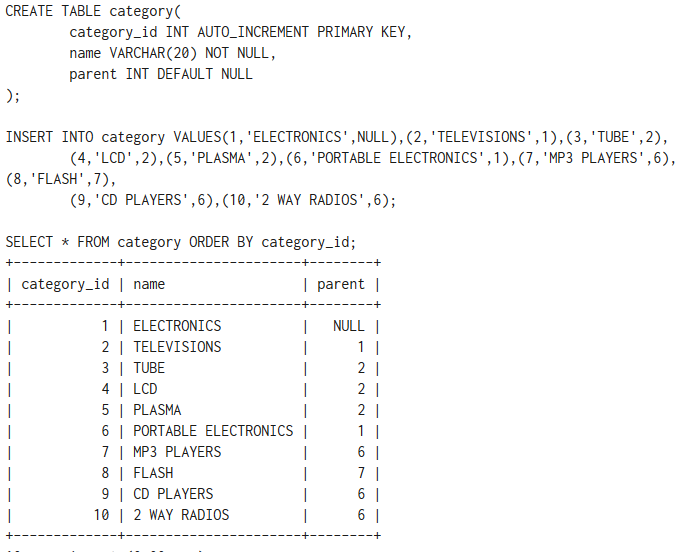
\includegraphics[scale=0.75]{images/Adjacency_list_model_table.PNG}
	\caption{Esempio di una tabella per gestire dati in modo gerarchico secondo l' adjacency list model }
\end{figure}
 
Il vantaggio di usare questo modello sta nella sua semplicità di costruzione sopratutto a livello di codice client-side, 
e di restituzione dei figli di un nodo. Mentre diventa problematico se si lavora in puro SQL e nella maggior parte dei linguaggi di 
programmazione, è lento e poco inefficente, perchè è necessaria una query per ogni nodo dell'albero, e visto che ogni query impiega 
un certo periodo di tempo, questo rende la funzione molto lente quando si lavora con alberi di grandi dimensioni.

\newpage

\subsection{The nested set model}
In the Nested Set Model, we can look at our hierarchy in a new way, not as nodes and lines, but as nested containers. 

\begin{figure}[ht!]
    \centering
	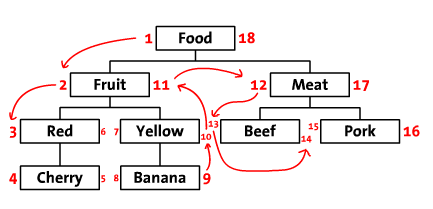
\includegraphics[scale=1]{images/Nested_Tree_Model_ex.PNG}
	\caption{Esempio di una gestione di dati in modo gerarchico secondo il modello innestato}
\end{figure}


We represent this form of hierarchy in a table through the use of left and right values to represent the nesting of our nodes, 
and indicate the relationship between each node.
So how do we determine left and right values? 
We start numbering at the leftmost side of the outer node and continue to the right. When working with a tree, we work from left to 
right, one layer at a time, descending to each node’s children before assigning a right-hand number and moving on to the right. 
This approach is called the modified preorder tree traversal algorithm.



OSS: Note that the words ‘left’ and ‘right’ have a special meaning in SQL. Therefore, we’ll have to use ‘lft’ and ‘rgt’ to identify 
the columns. Also note that we don’t really need the ‘parent’ column anymore. We now have the lft and rgt values to store the tree 
structure.

CONS: At first, the modified preorder tree traversal algorithm seems difficult to understand. It certainly is less simple than the 
adjacency list method. However, once you’re used to the left and right properties, it becomes clear that you can do almost everything 
with this technique that you could do with the adjacency list method, and that the modified preorder tree traversal algorithm is much 
faster. Updating the tree takes more queries, which is slower, but retrieving the nodes is achieved with only one query.


\section{Sistemi di raccomandazione}